\chapter{modello Circuitale}
\section{Modello Circuitale Elettrico}

\subsection*{Equazioni di Maxwell}
Le \textbf{Equazioni di Maxwell} permettono di studiare i fenomeni elettromagnetici e ottenere modellazioni precise del loro funzionamento.

\subsection*{Approccio Circuitale}
L'\textbf{Approccio Circuitale} serve a ottenere un modello semplificato di fenomeni.

\subsection*{Circuiti Elettrici a Costanti Concentrate}
I \textbf{Circuiti Elettrici a Costanti Concentrate} derivano da approssimazioni delle equazioni di Maxwell:

\begin{itemize}
    \item Dimensioni della struttura trascurabili
    \item Velocità di propagazione infinita
    \item Tempo nullo di trasmissione dei fenomeni
\end{itemize}

\textit{È ovviamente necessario verificare la validità delle approssimazioni.}

\begin{figure}[H]
    \centering
    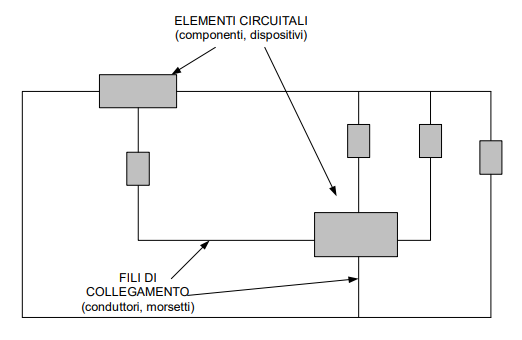
\includegraphics[width=0.7\textwidth]{capitoli/capitolo2/immagini/image1.png}
\end{figure}

\subsection*{Circuito a Costanti Concentrate}
Un \textbf{Circuito a Costanti Concentrate} è una connessione tra elementi ideali privi di dimensioni geometriche e caratterizzati da legami tra tensione e corrente.

\section{Grandezze Elettriche}

\subsection*{Tensione}
La \textbf{Tensione} è definibile tra due morsetti e si misura in \textit{Volt}. È necessario indicare intensità e verso. Il segno negativo indica inversione di polarità.

\subsection*{Corrente}
La \textbf{Corrente} è definibile su un morsetto e si misura in \textit{Ampere}. È necessario indicare intensità e verso. Il segno negativo indica inversione di direzione.

\begin{figure}[H]
    \centering
    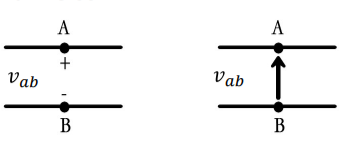
\includegraphics[width=0.7\textwidth]{capitoli/capitolo2/immagini/image2.png}
\end{figure}

\section{Porta Elettrica}

Una \textbf{Porta Elettrica} è costituita da una coppia di morsetti, con la relazione \(i' = i''\).

\subsection*{Grandezze di Porta}
Le grandezze associate alla porta sono \textbf{tensione} e \textbf{corrente}.

\subsection*{Potenza Istantanea}
La potenza istantanea si calcola come:
\[
p(t) = v(t) \cdot i(t) \quad \text{[Watt]}
\]

\subsection*{Versi}
Esistono due versi per la potenza istantanea:

\begin{figure}[H]
    \centering
    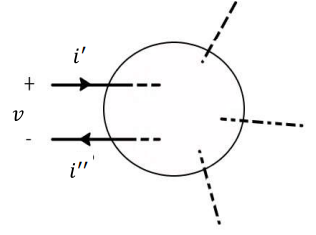
\includegraphics[width=0.7\textwidth]{capitoli/capitolo2/immagini/image3.png}
\end{figure}

\begin{itemize}
    \item \textbf{Porta dell’utilizzatore:} versi coordinati, potenza assorbita > 0.
    \item \textbf{Porta elettrica del generatore:} potenza assorbita < 0, versi non coordinati.
\end{itemize}

\section{Leggi di Kirchhoff}

\subsection*{Prima Legge di Kirchhoff (KLC)}
La somma algebrica delle correnti entranti e uscenti da una superficie chiusa è nulla. La superficie non può tagliare dei componenti, ma solo dei morsetti.

\begin{itemize}
    \item Correnti uscenti → segno +
    \item Correnti entranti → segno -
\end{itemize}

\begin{figure}[H]
    \centering
    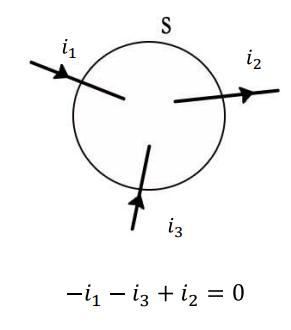
\includegraphics[width=0.7\textwidth]{capitoli/capitolo2/immagini/image4.png}
\end{figure}

\subsection*{Seconda Legge di Kirchhoff}
La somma algebrica delle tensioni lungo una curva chiusa è nulla. La curva chiusa non può tagliare dei componenti, ma solo dei morsetti.

\begin{itemize}
    \item Tensioni senso orario → segno +
    \item Tensioni senso antiorario → segno -
\end{itemize}

\begin{figure}[H]
    \centering
    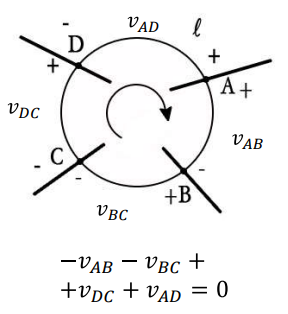
\includegraphics[width=0.7\textwidth]{capitoli/capitolo2/immagini/image5.png}
\end{figure}

\section{Componenti}

Un \textbf{Componente} è costituito da due o più terminali (poli). Un componente con N terminali è detto N-polo. Ad esempio, un bipolo è un componente con due poli.

\subsection*{Bipolo}
Un bipolo ha due morsetti che costituiscono una porta. Le grandezze elettriche sono \(v(t)\) e \(i(t)\). La relazione costitutiva di un bipolo completo è:
\[
f(v(t), i(t), t) = 0
\]
Un bipolo può essere pilotato in tensione o in corrente.

\subsubsection*{Pilotato in Tensione}
Se il bipolo è pilotato in tensione, la relazione è:
\[
i(t) = g v(v(t), t)
\]

\subsubsection*{Pilotato in Corrente}
Se il bipolo è pilotato in corrente, la relazione è:
\[
v(t) = g i(i(t), t)
\]

\subsection*{Potenza Istantanea}
La potenza istantanea per un bipolo è:
\[
p(t) = v(t) \cdot i(t)
\]

\subsection*{Versi Coordinati}
La potenza maggiore di zero viene effettivamente assorbita.

\begin{figure}[h!]
    \centering
    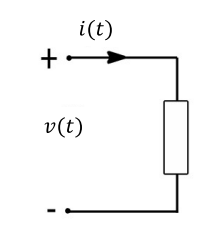
\includegraphics[width=0.7\textwidth]{capitoli/capitolo2/immagini/image6.png}
\end{figure}

\subsection*{Tripolo}
Un tripolo è un componente con tre terminali. La corrente in un tripolo è definita come la somma delle correnti nei terminali:
\[
i(t) = i_1(t) + i_2(t)
\]
Ogni coppia di morsetti può essere considerata come una porta elettrica.

\subsubsection*{2-porte sbilanciato}
Un tripolo può essere modellato come un sistema con due equazioni costitutive che legano le quattro grandezze di porta.

\subsubsection*{Potenza Istantanea}
La potenza istantanea per un tripolo è la somma delle potenze delle due porte:

\begin{figure}[H]
    \centering
    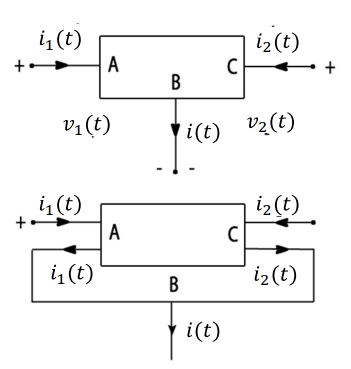
\includegraphics[width=0.7\textwidth]{capitoli/capitolo2/immagini/image7.png}
\end{figure}

\[
p(t) = v_1(t) \cdot i_1(t) + v_2(t) \cdot i_2(t)
\]

\subsection*{Quadripolo}
Un quadripolo è un componente con quattro terminali. La legge di Kirchhoff per le correnti (KLC) non pone vincoli particolari per un quadripolo.

\begin{figure}[H]
    \centering
    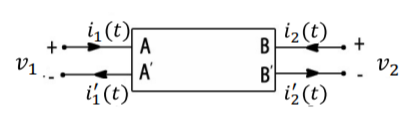
\includegraphics[width=0.7\textwidth]{capitoli/capitolo2/immagini/image8.png}
\end{figure}

\subsubsection*{2-porte Bilanciato}
Nel caso di un quadripolo bilanciato, la potenza istantanea è data da:
\[
p(t) = v_1(t) \cdot i_1(t) + v_2(t) \cdot i_2(t)
\]

\section{Ipotesi Aggiuntive}

\subsection*{Linearità}
Un sistema è lineare se l'effetto è proporzionale alla causa. La linearità permette l'uso del principio di sovrapposizione.
\[
e(t) \to \text{effetto dovuto alla causa } c(t)
\]
\[
a \to \text{costante}
\]

% Relazione tra c(t) e e(t)
\[
\text{*H*}: \text{Se } c(t) \xrightarrow{} e(t) \text{ allora } ac(t) \xrightarrow{} ae(t)
\]

% Conseguenza
\[
\text{*Conseguenza*}: 
\]
\begin{figure}[h!]
    \centering
    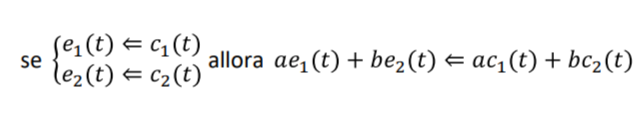
\includegraphics[width=0.7\textwidth]{capitoli/capitolo2/immagini/image9.png}
\end{figure}

\subsection*{Permanenza}
Un sistema è permanente se l'effetto non dipende dall'istante di applicazione della causa:
\[
c(t) \implies e(t) \quad \Rightarrow \quad c(t+t_0) \implies e(t+t_0) \quad \forall t_0 \text{ costante}
\]

\subsection*{Causalità}
Un sistema è causale se, in ogni istante \( t_0 \), l'effetto dipende solo dalla causa per \( t \leq t_0 \).

\begin{figure}[H]
    \centering
    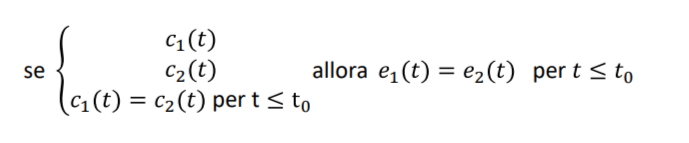
\includegraphics[width=0.7\textwidth]{capitoli/capitolo2/immagini/image10.png}
\end{figure}

\section{Proprietà Notevoli}

Le proprietà come \textbf{linearità}, \textbf{permanenza} e \textbf{causalità} devono essere soddisfatte in ogni sistema.

\subsection*{Reciprocità e Passività}
Le proprietà di reciprocità e passività possono essere verificate in un sistema.

\subsection*{Reciprocità}
La reciprocità implica che l'interazione tra due cause in un circuito non cambia se si scambiano ingresso e uscita.

\begin{figure}[H]
    \centering
    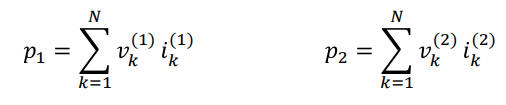
\includegraphics[width=0.7\textwidth]{capitoli/capitolo2/immagini/image11.png}
\end{figure}


\begin{figure}[H]
    \centering
    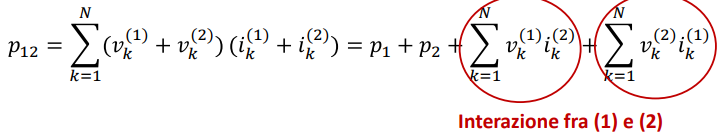
\includegraphics[width=0.7\textwidth]{capitoli/capitolo2/immagini/image12.png}
\end{figure}

\section*{Condizione di reciprocità}

\textbf{Legge di reciprocità di Lorentz}

In due situazioni elettriche diverse, un N-porte è reciproco se vale la condizione precedente.

Dato un componente lineare passivo:

\begin{enumerate}
    \item Si collega un generatore ideale di tensione in A e si considera la corrente di corto circuito in B: \( E_a I_b \)
    \item Si collega un generatore ideale di tensione in B e si considera la corrente di corto circuito in A: \( E_b I_a \)
\end{enumerate}

\textbf{Allora}: 
\[
\frac{E_a}{I_b} = \frac{E_a}{I_a}
\]

\textbf{E se}: 
\[
E_a = E_b \quad \text{e} \quad I_a = I_b 
\]
il comportamento del circuito non cambia scambiando ingresso e uscita.

\textbf{Passività}: L’effetto di una causa di breve durata scompare con il passare del tempo.

- È impossibile fornire energia (o al massimo minore di quella assorbita).

\[
t = -\infty \quad \Rightarrow \quad \text{circuito o componente a riposo}
\]

\subsection*{Passività}
Un sistema è passivo se l'effetto di una causa scivola nel tempo, senza fornire energia.

\section{Componenti Ideali}

\subsection*{Resistore}
Un resistore è misurato in \textit{Ohm} e segue la relazione:
\[
v(t) = R \cdot i(t)
\]

\subsection*{Condensatore}
Un condensatore ha una capacità misurata in \textit{Farad} e segue la relazione:
\[
i(t) = C \frac{d v(t)}{dt}
\]

\section*{Equazione Costitutiva}

\[
v(t) = R i(t) \quad \text{(R costante reale)}
\]

\[
R = \frac{v(t)}{i(t)}
\]

\[
G = \frac{1}{R} = \frac{i(t)}{v(t)} \quad \Rightarrow \quad i(t) = G v(t)
\]

\textbf{Condizione di passività:}

\textbf{Passivo} $\Rightarrow R \geq 0$ (componente reale)

\[
P(t) = R i^2(t) \geq 0 \quad \text{(trasferimento irreversibile di energia)}
\]

Allo zero assoluto è un superconduttore.

\textbf{Attivo} $\Rightarrow R < 0$

\[
P(t) = R i^2(t) < 0 \quad \text{(erogano energia)}
\]

\section*{Condensatore}

Capacità misurata in Farad.

\textbf{Componenti reali} sono caratterizzati dalla tensione di isolamento.

\[
i(t) = C \frac{d v(t)}{dt} \quad \text{(C costante reale)}
\]

\textbf{Passivo} $\Rightarrow C \geq 0$ (componente reale)

\textbf{Attivo} $\Rightarrow C < 0$

Componente con memoria.

\section*{Induttore}

Induttanza misurata in Henry.

\[
v(t) = L \frac{d i(t)}{dt} \quad \text{(L costante reale)}
\]

\textbf{Condizione di passività:}

\textbf{Passivo} $\Rightarrow L \geq 0$

\textbf{Attivo} $\Rightarrow L < 0$

Componente con memoria.

\section*{Generatore Indipendente di Tensione}

Ingresso al circuito.

L'energia può assumere qualsiasi valore.

Componente attivo.

\[
v(t) = V_g(t) \quad \text{(funzione del tempo, eventualmente costante)}
\]

Cortocircuito: $v_g(t) = 0$

\section*{Generatore Indipendente di Corrente}

Ingresso al circuito.

\[
i(t) = i_g(t)
\]

L'energia può assumere qualsiasi valore.

Componente attivo.

Circuito aperto: $i_g(t) = 0$

\section*{Circuiti Equivalenti dei Bipoli Reali}

E' necessario modellare il componente reale considerando altri elementi ideali.

L'inserimento di una resistenza elimina l'assurdo.

\textbf{Resistori in serie}: percorsi dalla stessa corrente $i$.

\textbf{Partitore di tensione}: la tensione si ripartisce su più resistori in maniera proporzionale alle resistenze.

\textbf{Resistori in parallelo}: ai capi hanno la stessa tensione.

\section*{Connessione di Bipoli}

\textbf{Partitore di corrente}: la corrente si ripartisce in maniera inversamente proporzionale alle resistenze.

\section*{Componenti Ideali}

\textbf{2-porte}:

\begin{itemize}
    \item Tripolari o quadrdipolari.
    \item Non sempre hanno un equivalente componente reale.
    \item Utili per circuiti più complessi.
    \item Generatori controllati: elementi attivi, non reciproci, si possono realizzare tutti i 4 tipi da uno solo.
\end{itemize}


\textbf{Nullore}: possono assumere valori qualsiasi, poco realistico, attivo e non reciproco.

\textbf{Trasformatore ideale}: non assorbe potenza, senza perdite, passivo, reciproco.

\textbf{Induttori manualmente accoppiati}: trasferimento reversibile vincolato di energia, componente con memoria.

\textbf{Giratore}: non assorbe potenza, senza perdite, passivo, non reciproco.
